\documentclass[%
  a4paper,oneside,%
  arial,
  11pt,% <10pt, 9pt>
  %smallchapters,
  %style=screen,
  %sender=bottom,
  green,% <orange, green, violet>
  rgb, <cmyk>
  %mono
  ,]{tubsbook}
\usepackage[utf8]{inputenc}

\usepackage[ngerman,english]{babel}

\usepackage{lipsum} % Blindtext-Paket
\definecolor{InAGreen}{RGB}{172,193,58}

% Titelseiten-Elemente
\title{Beispieltitel}
\subtitle{Untertitel}
\author{Max Mustermann}
%\logo{Institut fuer Lorem Ipsum}
\logo{
\includegraphics{InA-Logo-rgb.pdf}}
\titleabstract{\lipsum[2]}
\titlepicture{infozentrum.jpg}
% Rückseiten-Elemente
\address{%
  Herr Mustermann\\
  Schlossallee 1\\
  33333 Darmstadt}
\backpageinfo{%
  \lipsum[5]
}
\usepackage{pdfpages}								% Einbinden von PDF-Pages
\usepackage[colorlinks,pdfpagelabels,pdfstartview = FitH,bookmarksopen = true,bookmarksnumbered = true,linkcolor = black,plainpages = false,hypertexnames = false,citecolor = black] {hyperref}
\usepackage[figure]{hypcap} 
\bibliographystyle{ieeetr}

\begin{document}

%\maketitle[image,logo=left]%[<plain/image/imagetext>,<logo=left/right>]
%\makebackpage[trisec]%[<plain/info/addressinfo>]
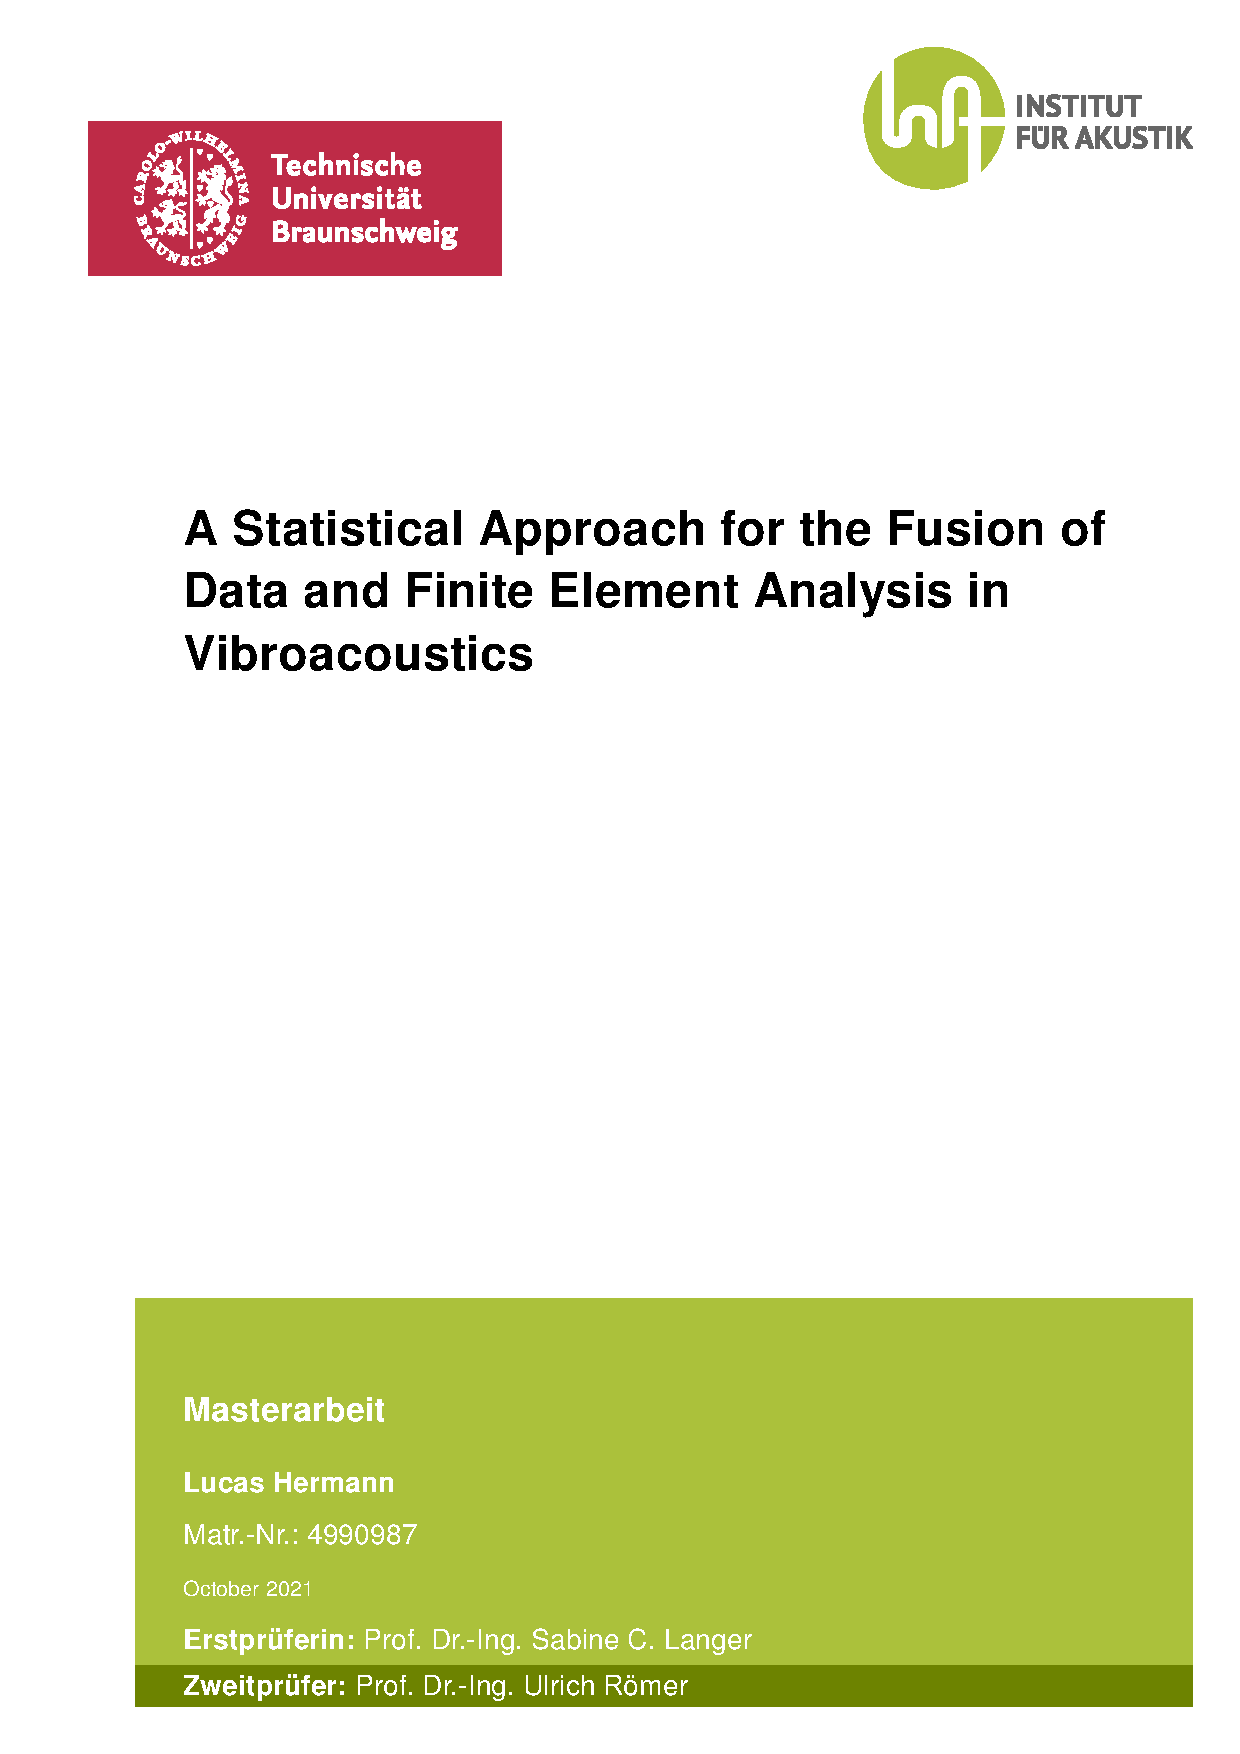
\includepdf[pages=-]{./Deckblatt/2099_StA_Name_Deckblatt.pdf}

\chapter*{Declaration}
Hiermit versichere ich, <Vorname> <Nachname>, durch meine Unterschrift, dass ich die
vorliegende Masterarbeit mit dem Titel ``<<Titel>>'' selbständig und ohne Benutzung
anderer als der angegebenen Hilfsmittel angefertigt habe. Alle Stellen, die wörtlich oder sinn-
gemäß aus veröffentlichten oder unveröffentlichten Schriften entnommen sind, habe ich als
solche kenntlich gemacht. Insbesondere sind auch solche Inhalte gekennzeichnet, die von
betreuenden wissenschaftlichen Mitarbeiterinnen und Mitarbeitern des Instituts für Akustik eingebracht wurden.

Die Arbeit oder Auszüge daraus haben noch nicht in gleicher oder ähnlicher Form dieser
oder einer anderen Prüfungsbehörde vorgelegen.

Mir ist bewusst, dass Verstöße gegen die Grundsätze der Selbstständigkeit als Täuschung
betrachtet und entsprechend der Prüfungsordnung geahndet werden.

\begin{flushright}
Braunschweig, \today
\end{flushright}

\vspace{2cm}
\hspace{2cm}\rule{5cm}{1pt}

\hspace{2cm}\small{Vorname Nachname} 

\chapter*{Abstract}
\lipsum[1]

\tableofcontents


\chapter{Chapter 1}

\textcolor{tubsSecondary}{Dies ist ein Text in \texttt{tubsSecondary}.}
\textcolor{tubsViolet}{Dies ist ein Text in \texttt{tubsViolet}.}
\textcolor{tubsGreenDark}{Dies ist ein Text in \texttt{tubsGreenDark}.}\bigskip

\lipsum[1]

\begin{itemize}
  \item Aufzählungspunkt Eins
  \item Aufzählungspunkt Zwei
    \begin{itemize}
      \item Unter-Aufzählungspunkt Eins
      \item Unter-Aufzählungspunkt Zwei
    \end{itemize}
  \item Aufzählungspunkt Drei
\end{itemize}

\chapter{Chapter 2}

\lipsum[2-5] %\cite{campolina}

\chapter{Chapter 3}

\lipsum[1-3] %\cite{Langer2019}

\section{Section 1}

\lipsum[4-7] %\cite{Yaghoubi:2017}


\begin{thebibliography}{4}
%
\bibitem{campolina}
Campolina, B.: Vibroacoustic modelling of aircraft double-walls with structural links using Statistical
Energy Analysis (SEA). Acoustics [physics.class-ph]. Université de Sherbrooke; Université Pierre
et Marie Curie - Paris VI (2012)

\bibitem{Langer2019}
Langer, S.C., Blech, C.: Cabin noise prediction using wave‐resolving aircraft models. Proc. Appl. Math. Mech., Vol. 12 (1) (2019): e201900388. doi:10.1002/pamm.201900388

\bibitem {Yaghoubi:2017} Yaghoubi, V., Marelli, S., Sudret, B., Abrahamsson, T.: Sparse polynomial chaos expansions of frequency response functions using stochastic frequency transformation, Probabilistic Engineering Mechanics, volume 48, pages 39-58 (2017)
\end{thebibliography}

\end{document}
